\chapter{DAH Checkpoints}
\label{sec:checkpoints}
\vspace*{-0.99cm}
{\bf Important note}: Please consult the DAH manual to familiarise yourself with the equipment, including the Raspberry-Pi, LED and temperature sensors, ADCs, DACs, I/O, switches, breadboard and connectors. The manual contains details instructions how to operate the Raspberry-Pi. It is suggested to use the epiphany browser on the Raspberry Pi. To copy python code snippets, see below, into your python scripts download these files from github, see \url{https://github.com/fmuheim/DAH}.  Data sheets for all electronic elements, are available from Dropbox,
see: \url{https://www.dropbox.com/sh/gfnisnh4ntnum1d/AAAWtNL_AhcpR8PZ_QmqZpsja?n=112609310}.  
The DAH manual also provides information on how to start and stop the \webIOPi Code application.

\section{Checkpoint  1: LEDs and Switches}

\begin{enumerate}
\item [1.1.] Control and LED with the Raspberry-Pi by completing the following steps. Connect the Raspberry-Pi to a breadboard and start the \webIOPi Code application.
Start the epiphany web browser and %on the Raspberry Pi and go to \url{localhost:8000}.
go to the \webIOPi header webpage, set GPIO 24 to OUT, connect this output to a LED with a 1~kOhm resistor in series to ground, switch the LED on and off.  Repeat the exercise with negative logic (active low) by connecting the LED with a 1~kOhm resistor in series to 3.3 V.  Draw a schematic diagram for this circuit, see example below.  

\hfill [2 marks]
 \vspace*{-8mm}
 \begin{center}                                        
 {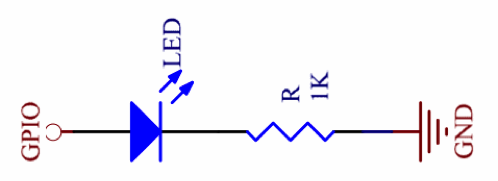
\includegraphics[width=10cm]{figs/ActiveHighLED}}
 \end{center}
                                                            
 
\item [1.2.] Using positive logic (active high) connect a push-button Switch between 3.3V and GPIO23 and, with a 1kOhm resistor in series, to ground and explain what happens on the webIOPI header webpage. Draw a schematic diagram for this circuit. Afterwards stop the  \webIOPi Code application.
%Repeat the exercise with negative logic, explain it and draw a schematic diagram. 
 
 \hfill [1 mark]\\
      

\item [1.3.]  Connect an LED with a 1~kOhm resistor as in checkpoint 1.1 above. Start python interactively to set GPIO 24.   Using the templates, import the webiopi framework, make a GPIO object and turn the LED on and off.
%
\begin{verbatim}
    studentn@dahpimm  ~ $ sudo python3
\end{verbatim}
\lstinputlisting{../scripts/checkpoint_1a.py}


Write the first Python script to blink an LED for either positive or negative logic 
by adding a "while loop".\\

\lstinputlisting{../scripts/checkpoint_1b.py}
\vspace*{-0.5cm}
\hfill [2 marks]\\


\item [1.4.]	  Connect the push button switch using  using negative logic (active low)  and the LED circuit with positive logic (active high).  Write a python script to toggle the LED status every time the push button switch is pushed. \\
%once using negative logic for the push button switch. Connect the push and positive logic for the LED. \\

\lstinputlisting{../scripts/checkpoint_1c.py}
\vspace*{-0.5cm}
\hfill [2 marks]\\


\end{enumerate}



\newpage
\section{Checkpoint 2: ADC, DAC and  SPI BUS}

\begin{enumerate}

\item [2.1.]	 Connect Analog-to-Digital Converter (ADC) MCP3208 chip to the Raspberry-Pi using the SPI Interface on pin GPIO 8 (SPI\_CE0). Make sure that all required connections between the MCP3208 and the Raspberry-Pi are made, see the pin-out sheet. Use a multimeter to check that power (VDD) and ground (AGND and DGND) are correctly connected. Explain what all connections are for?

Connect a potentiometer between 3.3 V and ground and connect the output to one of the ADC input channels.  Use python interactively to read the voltages of all eight channels. Play with changing the input channel(s).  Read the ADC channels using all the methods given below. You are encouraged to consult the following webpage where you also can find this information, see \url{http://webiopi.trouch.com/} ($\rightarrow$ Tutorials $\rightarrow$ Using Devices $\rightarrow$ Analogue). Explain how the ADC works and what the meaning of the return values of each method is. What is the primary ADC output and how is the voltage output calculated from this? \\

\lstinputlisting{../scripts/checkpoint_2a.py}
\hfill [3 marks]\\

\newpage
\item [2.2.]	 Connect the Digital-to-Analog-Converter (DAC) MCP4922 chip to the Raspberry-Pi using the SPI Interface on GPIO 7 (SPI\_CE1). Make sure that all required connections between the MCP4922 and the Raspberry-Pi are made, see pin-out sheet. Use a multimeter to check that power (VDD) and ground (AVSS) are correctly connected. Explain and how the DAC works and what all connections are for. 

Use python interactively to set a value, e.g. 1.3 V to output VOUTA of the DAC. Measure this voltage with a multimeter. \\

\lstinputlisting{../scripts/checkpoint_2b.py}
\hfill [2 marks]\\

\item [2.3.] Connect the two outputs of the DAC MCP4922 to two inputs of the ADC MCP3208. Write a python script that that sets a series of different values on both two DAC outputs and reads the corresponding values of the ADC channels.  Write the DAC setting and measured ADC values at each step to an output file with comments such that the content of the file will explain your work.  

\hfill [3 marks]\\

\end{enumerate}



\newpage
\section{Checkpoint 3:  Generating and Sampling Analogue Signals}

\begin{enumerate}

\item [3.1.] Connect an ADC chip (MCP3208) to the Raspberry Pi, as in Checkpoint 2. Verify that the ADC works with a DC voltage produced with a potentiometer.

Use the signal generator to produce a repetitive signal, e.g. a sinusoidal waveform. Display the output on the oscilloscope. Set the amplitude of the signal such that the waveform can be read by the ADC chip, which can sample between 0 V and VREF = 3.3 V. Set the frequency to 10 Hz.  

Connect the output of the signal generator to an ADC input channel. Using python in interactive mode read a few samples of the ADC output. Comment on what you measure. [Caveat: Don't connect a signal with a voltage outside the range of the ADC chip, which could destroy it and the Raspberry Pi.] 

\hfill [1 marks]\\

\item [3.2.] Measure the waveform produced by the signal generator by writing a python script that records 100 ADC samples and displays these on a graph. Always label plots correctly with title and axes and save these to a file (pdf format). 
[Hint: Use the pylab interface for plotting graphs as discussed in the python tutorial. Example files are available on github. ]

\hfill [2 marks] \\

\item [3.3.] Calibrate the voltage scale of the ADC output with respect to the oscilloscope by using a square waveform that matches the ADC input range.  First connect the signal from the signal generator to the oscilloscope and read the input voltage for the high and low sections of the square waveform off the oscilloscope screen. (Use the trigger threshold dial to determine these quite precisely). Then connect the signal to an ADC input channel. Write a python script that takes 100 ADC samples and writes these onto the screen or into a file. Determine the average ADC values for the high and low sections of the square waveform and plot these versus the two input voltages. Reduce the amplitude of the input waveform by a factor of two and repeat above procedure.  Plot the four calibration measurements on a graph and comment.

\hfill [2 marks] \\

\item[3.4.]	What is the maximum signal frequency with which you can properly record a given repetitive signal?  Consider which would be the best waveform for this investigation. What is the sampling frequency? Explain what happens when a signal is undersampled. Make a plot with a waveform that is undersampled.   

\hfill [2 marks] \\

\item [3.5.] Connect a DAC chip (MCP4922) to the Raspberry Pi, as in Checkpoint 2.  Using a python script, generate a sinusoidal waveform on the DAC output and plot the waveform to a graph.

Use the ADC chip (MCP3208) to digitise the waveform generated by the DAC. Write a python script that takes 100 DAC samples and 100 ADC measurements and plot these on the same graph. Take into account the limitations encountered in 3.4.                                                          
 
\hfill [3 marks] 

\end{enumerate}


\newpage
\section{Checkpoint 4: Input/Output I/O and I2C BUS}

\begin{enumerate}


\item [4.1.] Input/Output (I/O) Expander chips enable the user to connect many devices having the same or similar functions.  With the Raspberry Pi this can be achieved using the I2C bus. Connect the PCF8574AN chip  (I2C BUS Expander) to the Raspberry-Pi. Make sure that all required connections between the PCF8574AN chip and the Raspberry-Pi are made, see pin-out sheet. Explain how the I/O Expander works and what the SDA, SCL and A0, A1, A2 address lines are. 
%\hfill [2 marks]\\

%\item [4.2.] 
Using negative logic connect an LED to output P0 of the PCF8574AN Expander chip. 
Write a python script to blink the LED using negative logic, see checkpoint 1 for setting up a while loop.  Why is negative logic necessary? 

You may consult the \webiopi webpage  \url{http://webiopi.trouch.com/} ($\rightarrow$ Tutorials $\rightarrow$ Using Devices $\rightarrow$ Digital) to find information on the GPIO expander chip. \\

\lstinputlisting{../scripts/checkpoint_4a.py}
\hfill [3 marks]\\

\item [4.2.] Connect an additional 3 LEDs to outputs P1, P2 and P3 of the PCF8574AN Expander chip. Write a python script which turns the LEDs on and off in a predefined pattern, such as a running light. Consider P0 to P3 as default, but you are encouraged to play with other patterns. 

\hfill [2 marks]\\

\newpage
\item [4.3.] Consult the webpage \url{http://webiopi.trouch.com/} ($\rightarrow$ Tutorials $\rightarrow$ Using Devices $\rightarrow$ Digital) for the GPIO Expander. Use the portWrite(value) method to manipulate all four LEDs at the same time.  Connect a push button switch to pin P4 of the expander chip. Write a python script such that an LED pattern toggles every time the button is pushed.\\

\lstinputlisting{../scripts/checkpoint_4b.py}
\hfill [3 marks]\\


\end{enumerate}



\newpage
\section{Checkpoint 5: Temperature Sensors}

\begin{enumerate}

\item [5.1.] We will be using DS18B20 temperature sensors for this checkpoint. Take a look at the datasheet here: http://www.adafruit.com/datasheets/DS18B20.pdf  or download it from the DAH Dropbox.

Connect a DS182B0 temperature sensor to your Raspberry pi (look at the flat front of the sensor to get it the right way around):
\begin{center}
    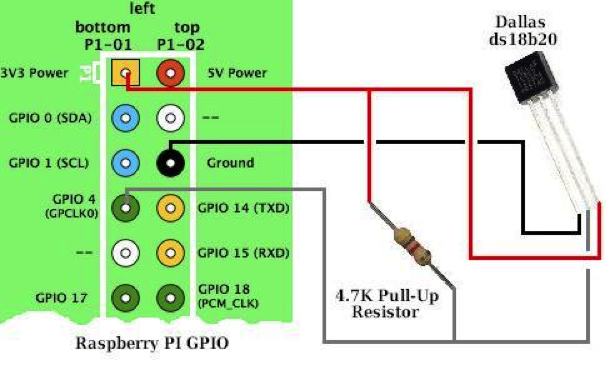
\includegraphics[width=14cm]{figs/DS182B0}
\end{center}

What is the interface between the DS18B20 temperature sensor and the Raspberry Pi? Explain how it works. 

\begin{comment}
Install the drivers for the sensor on the Raspberry Pi with the following commands:
    pi@Demonstrator-pi ~ $   sudo modprobe w1-gpio
    pi@Demonstrator-pi ~ $   sudo modprobe w1-therm

Note that you will need to do this again if you restart the Raspberry Pi.
\end{comment}

Locate the sensor output by finding the file that has the serial number of your sensor:
\begin{verbatim} 
    studentn@dahpimm ~ $  cd /sys/bus/w1/devices 
    studentn@dahpimm /sys/bus/w1/devices $ ls 
    10-00080265b6d6 w1_bus_master1 
\end{verbatim}
where n = 1 to 50 and mm = 01 to 22.
Note that your temperature sensor won't be called 10-00080265b6d6, this is just an example.

Now read the sensor output, i.e. the raw temperature measurement:
\begin{verbatim}
    studentn@dahpimm /sys/bus/w1/devices ~ $ cd 10-00080265b6d6
    studentn@dahpimm /sys/bus/w1/devices/10-00080265b6d6 $ cat w1_slave 
    30 00 4b 46 ff ff 0d 10 29 : crc=29 YES 
    30 00 4b 46 ff ff 0d 10 29 t=23937 
\end{verbatim}
    
This should be interpreted as 23.937 centigrade (degree Celsius). 

\newpage
WebIOPi provides a simple way to access the temperature sensor data in python. It is best to test this by running python in interactive mode first.  
\begin{verbatim}
    studentn@dahpimm ~ $ python3
\end{verbatim}
\lstinputlisting{../scripts/checkpoint_5a.py}
\hfill [2 marks]


\item[5.2.] Measure temperature with the DS18B20 sensor versus time. Choose a sensible time interval. Write a python script to make a graph of 50 temperature measurements versus time. Always label plots correctly with title and axes and save these to a file.
 
As a second step the graph should update itself as each temperature measurement is made. Write a python script for this purpose.  Once this is working, play with it by touching the temperature sensor with you fingers. Describe what is happening and sketch it in your lab book.

You should probably use the following python commands:\\

\lstinputlisting{../scripts/checkpoint_5b.py}
\hfill [3 marks]



\item[5.3.]	Add another temperature sensor to your circuit by connecting it in parallel with the existing one. You don't need to make separate connections to the Raspberry Pi: your new sensor can share these with the existing one (Just make sure that you connect it the right way around).

Find its serial number in the w1/devices folder like before. Now ensure that you can read out your two temperature sensors simultaneously in python. You can test this by running python in interactive mode first. 
Note that your temperature sensors will have different serial numbers.

\begin{verbatim}
    studentn@dahpimm  ~ $ python3
\end{verbatim}
\lstinputlisting{../scripts/checkpoint_5c.py}

What is the smallest change in temperature that a sensor can report? Explain this with reference to the datasheet, and how the temperature information is encoded.

Investigate the accuracy of the sensor readings by looking at the stability of the measurement with time, and by comparing the outputs of your two sensors. You can probably assume that the ambient temperature in the lab is constant, but shielding your sensors from breezes may help.

Modify your graphing code from part 5.2 to make histograms of the temperature measurements of the two sensors. 

You can use the pylab histogram command:\\
\lstinputlisting{../scripts/checkpoint_5d.py}
Make also a graph of the difference between the temperature of the two sensors. Determine the RMS value of a set of temperature difference measurements between the two sensors. Explain your results. Are these consistent with the datasheet?

\hfill [3 marks]


\end{enumerate}


\newpage
\section{Checkpoint 5: Data Handling and Analysis}

\begin{enumerate}

\item [6.1.] This is a data handling exercise and the Raspberry Pi is not required.
Thus this checkpoint is best carried out using the Physics CPlab computers. 
There is a CPlab computer available on every desk in the DAH laboratory.
You can use the following python libraries. \\

\lstinputlisting{../scripts/checkpoint_6a.py}

The LHCb experiment at the Large Hadron Collider at CERN has recorded a sample of muon pairs with invariant masses in the range of 8.5 to 11 GeV/$c^2$. Three clear peaks are observed in this mass spectrum. These correspond to the production of Upsilon mesons, which are bound states of a $b$ and a anti-$b$ quark. These states are known as the $\Upsilon \rm (1S)$, $\Upsilon \rm (2S)$ and $\Upsilon \rm (3S)$ mesons where the $\Upsilon \rm (1S)$ meson is the ground state and the $\Upsilon \rm (2S)$  and $\Upsilon \rm (3S)$  states are radial excitations (for LHCb paper, see {DOI: 10.1007/JHEP06(2013)064).}

\begin{center}
    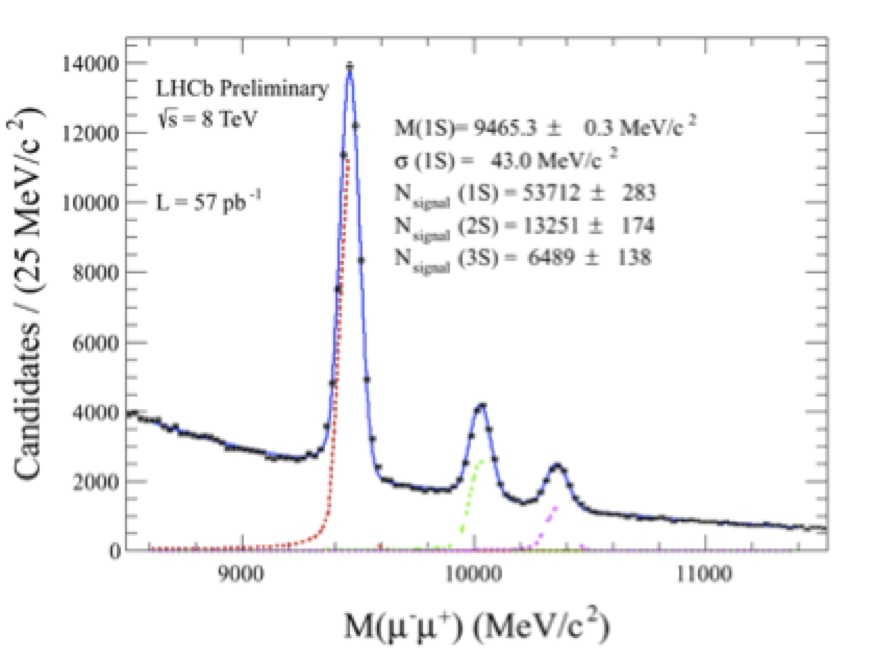
\includegraphics[width=9cm]{figs/mu-pair-mass}
\end{center}

Download the file upsilons-mass-xaa.txt from the DAH Dropbox, which contains the invariant masses of a large number of muon pairs in units of GeV/$c^2$ in text format. Write a python script that reads the data from this file and plots a histogram of all the masses, choosing a reasonable bin width. Always label plots correctly with title and axes and save these to a file.
[Hint: The bin width should be chosen such that each of the three peaks is clearly resolved and represented by a sufficient number of bins for analysis.]

\hfill [2 marks]


\item [6.2.] Determine the masses of the three particles by determining the bins with the highest number of entries in the peak regions. Divide the histogram into three peak regions and write a local peak finding method for this part.
What are the mass differences between the $\Upsilon \rm (2S)$ and $\Upsilon \rm (3S)$ states with respect to the $\Upsilon \rm (1S)$ meson? By inspecting visually the muon-pair mass
spectrum, determine the Full Width Half Maximum (FWHM) of the $\Upsilon \rm (1S)$ mass peak.

\hfill [2 marks]


\item [6.3.] Determine the mass of the  $\Upsilon \rm (1S)$  meson and its statistical uncertainty. This can be achieved by several methods. First by looking at the mass spectrum, choose a suitable region around the $\Upsilon \rm (1S)$  mass peak. Calculate the mean, the unbiased variance and standard deviation for the events in this region. Use these values to determine the standard deviation of the mean. Comment on possible biases for this method. 


The mass peaks corresponding to the three $\Upsilon$ mesons can be described 
reasonably well by a Gaussian function, 
$f(x) = \frac{N}{\sigma \sqrt{2\pi}}  \exp{\left( - \frac{(x-/\mu)^2}{2\sigma^2} \right)} $
where $x$ is the invariant mass of the muon pairs, $\mu$ is the mass of the $\Upsilon \rm (1S)$  meson, $\sigma$ is the Gaussian width (mass resolution) and $N$ is the total number of signal events. 
Estimate the mass resolution $\sigma$ from the FWHM of the $\Upsilon \rm (1S)$  peak. Compare the mass resolution with the standard deviation in the signal region determined above.

\hfill [2 marks]\\


In the muon-pair mass spectrum define a signal region of width $\pm 150\; {\rm MeV}/c^2$ around the $\Upsilon \rm (1S)$  peak position and determine the number of events $N$ in this region. 
Define an upper and lower sideband region where there are only background events. These sidebands should each be half as wide as the signal region and located at masses equidistant from the $\Upsilon \rm (1S)$  peak position. Assuming that the background is falling linearly with the muon-pair mass, determine the number of background events $B$ in the signal region (below the $\Upsilon \rm (1S)$  mass peak). Perform either a linear least squares fit in the sideband regions or use the sideband subtraction method for this. Determine the number of signal events $S$ in the signal region.

Alternatively, if you know how to perform a fit you may choose fitting the $\Upsilon \rm (1S)$   peak in the mass spectrum for this part.

% Assuming Gaussian statistics for N and using the mass resolution ? determine the statistical error %on the mass of the ?(1S) meson. 
Compare your mass measurement with the Particle Data Group (\url{pdg.lbl.gov}) and comment.
[Hint: The PDG lists the properties of particles. Select "pdgLive - Interactive Listings" followed by "Mesons b anti-b" to find the $\Upsilon \rm (1S)$  meson.]

\hfill [3 marks]

\begin{comment}

6.4. Download the file upsilons-mass-pt-xaa.txt from the DAH Dropbox which, in addition to the masses, also contains the transverse momenta pT of the muon- pairs in units of GeV/c in text format. For an explanation of the transverse momentum, see the LHCb paper, referred to above. Write a python script that reads in these data and plot a histogram of the transverse momenta for all events. Plot a 2-dimensional histogram of pT versus mass for all events, choosing 50 bins in pT and 100 bins in mass.
[Hint (python):]
%# Splitting a line with two strings separated by a blank space line = line.split()
12
[1 mark]

\end{comment}



\end{enumerate}
